\chapter{IMPLEMENTATION} \label{chap:implementation}

This chapter shows an implementation of Isenberg Dynamics and \algname{} together to compute the constraints of a second-order CBF. The main object used in this implementation is the \textit{Link}, used to store the mass properties, as well as the local position of a body in an open kinematic chain. A link is a 9 - tuple  defines as the following.

\begin{align} \label{eqn:link_tuple}
    l_B = \begin{pmatrix}
        B \in \mathbb{N} & 
        p \in \mathbb{L} \union \cup \emptyset &
        ^{B-1}\T_B \in \mathbb{R}^{3 \times 3} &
        ^{B-1}_{B-1}\r_B \in \mathbb{R}^3 \\
       \IHat_B \in \mathbb{R}^{3 \times n} &
       \ITilde_B \in \mathbb{R}^{3 \times n} &
       m_B \in \mathbb{R} &
       \BB\com \in \mathbb{R}^3 &
       \BB\J \in \mathbb{R}^{3 \times 3} 
    \end{pmatrix}
\end{align}
\noindent where
\begin{align*}
\begin{split}
    B &\equiv \text{Index in state vector} \\
    p &\equiv \text{Parent link} \\
    ^{B-1}\T_B &\equiv \text{Local Rotation Matrix} \\
    ^{B-1}_{B-1}\r_B &\equiv \text{Local Position Vector} \\
\end{split}
\begin{split}
    \IHat_B &\equiv {\BB\omega_{\mathbf{B-1}}} = \IHat_B\dotx  \\
    \ITilde_B &\equiv \mathbf{^{B-1}_{B-1}}\dotr_{\mathbf{B}} = \ITilde_B\dotx  \\
    m_B &\equiv \text{Mass} \\
    \BB\com &\equiv \text{Center of Mass} \\
    \BB\J&\equiv \text{Inertia Tensor} 
\end{split}
\end{align*}
\noindent For links without a parent, the convention is to model them as though they are attached to an immobile link of infinite mass, i.e. the Inertial Reference Frame link. In an implementation, this allows one to use the same recursive function calls for root links as they would for non-root links, rather than writing a special case for the root.


\section{Algorithms}

\noindent For each link in a system, the implementations of dynamics and \algname{} are each split into two stages representing the Kinematics and Dynamics portions of their computation. 

\begin{figure}[H]
    \centering
    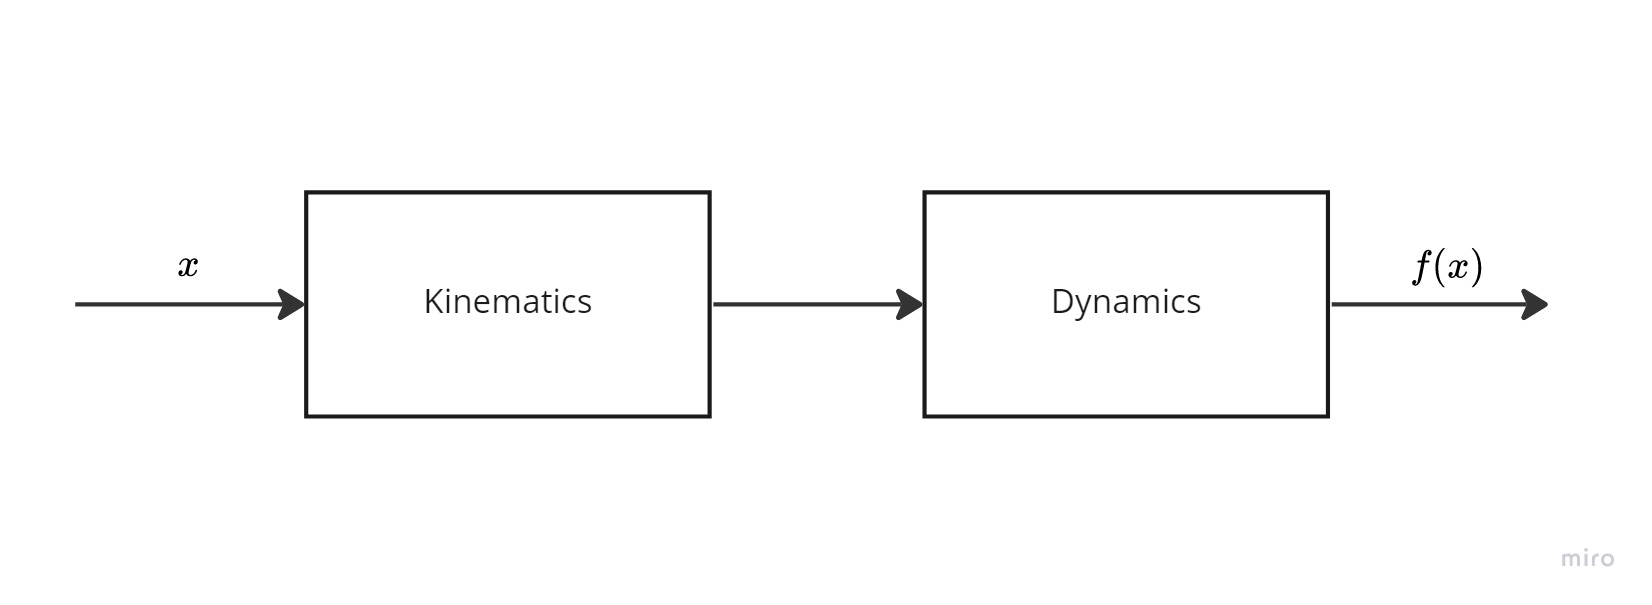
\includegraphics[width=\textwidth]{Figures/Implementation/IsenDynamcs.jpg}
    \caption{Dynamics}
    \label{fig:isendyn}
    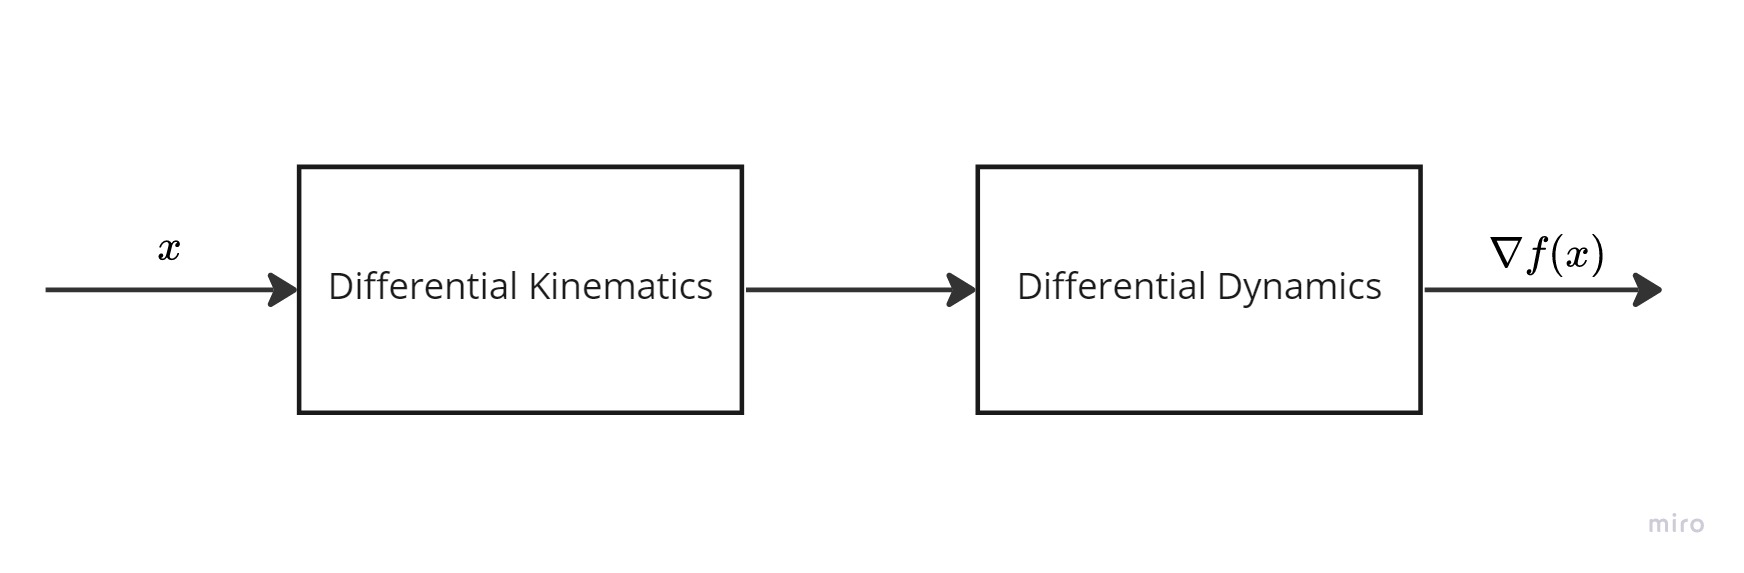
\includegraphics[width=\textwidth]{Figures/Implementation/GradDynamics.jpg}
    \caption{\algname{}}
    \label{fig:graddyn}
\end{figure}

\noindent While this could be done purely to follow the best practices of writing small, concise functions, there are some performance gains worth mentioning as well. Such a split across these stages allows the potential of a rudimentary parallel pipeline, as the dynamics stage does not depend on any information from the previous link. Thus, one could run the dynamics step of link $B-1$ during the kinematics step of link $B$. It also allows the kinematics stages to easily be skipped for the Inertial Reference Frame link, which is assumed to be unmoving and thus does not need to update its Kinematics. \newpage

Algorithms \ref{alg:kinematics} - \ref{alg:diff_dynamics} show the complete description for each of these procedures.
 
\begin{algorithm}[H]
	\caption{Kinematics}\label{alg:kinematics}
	\begin{algorithmic}
		\If{$t_\B$  = rotational}
		\State ${\BL}\T_\B \gets {^\mathbf{B-1}}\T_{\B_0}\cdot$axang($\x_i , \IHat_{B_i}$)
		\Else
		\State ${\BL}\T_\B \gets {^\mathbf{B-1}}\T_{\B_0}$
		\EndIf
		\State $\BL\r_\B \gets {\BL}\r_{\B_0} + \ITilde_{B_i}\x_i$
		\State $^I\T_\B \gets {^I\T_{\B-1}}{^{\B-1}}\T_\B$
		\State $\BB\omega_{\B -1 } \gets \IHat_{B_i} \dotx_i$
		\State $\BL\dotr_{\B} \gets \ITilde_{B_i} \dotx_i$
		\State $\J_\B' \gets  \begin{bmatrix}
		{^B\T_{B - 1}}                                       & \ZERO_{3 \times 3} \\
		\left (\S{^{B-1}_{B-1}\r_B}{^{B-1}\T_{I}} \right )^T & \EYE_{3 \times 3}  
		\end{bmatrix}$
		\State $\J_\B \gets \J_\B' \J_{B-1} + \begin{bmatrix} 
		{\IHat_\B} \\
		{{^I\T_{\B-1}}\ITilde_\B}
		\end{bmatrix}$
		\State $\dotJ_\B'' \gets (\S{^{B-1}_{B-1}\omega_I}\S{^{B-1}_{B-1}\r_\B}+\S{^{B-1}_{B-1}\dotr_\B)}$
		\State $\dotJ_\B' \gets \begin{bmatrix}  
		-\S{\BB\omega_{B-1}}{^B\T_{B-1}}                                       & \ZERO_{3 \times 3} \\
		-{^I\T_{B-1}}
		\dotJ_\B'' & \ZERO_{3 \times 3} \\
		\end{bmatrix}$
		\State $\dotJ_\B \gets \dotJ_\B' \J_{B-1} + \J_\B' \dotJ_{B-1} + \begin{bmatrix} 
		\ZERO_{3 \times n} \\
		{{^I{\T}_{B-1}}\S{^{B-1}_{B-1}\omega_I}\ITilde_\B} \\
		\end{bmatrix}$
	\end{algorithmic}
\end{algorithm}

\begin{algorithm}[H]
	\caption{Dynamics}\label{alg:dynamics}
	\begin{algorithmic}
		\State $\M' \gets \S{m_\B {\BB}c}{^\B\T_I}$
		\State $\M_\B \gets \begin{bmatrix}{\BB\J} & \M' \\ {\M'}^T & m_\B\EYE_{3 \times 3}\end{bmatrix}$
		\State $\H_\B = \J_\B^T \M_\B \J_\B$
		\State $\d_\B' \gets \begin{bmatrix}                            
		{\BB\omega_I } \times (\BB\J \times {\BB\omega_I}) \\
		{^I\T_\B}  (\BB\omega_I \times (\BB\omega_I \times \com))\\
		\end{bmatrix}$
		\State $\d_\B  \gets \J^T_\B \left (\M_\B \dotJ_\B + \d'_\B \right)$
		\State $\F_{B_J} \gets \Big.\sum_{\mathbf{\hat{K}_i} \in \mathbf{\hat{K}}}\mathbf{\hat{K}_i(\x, \dotx)} $
		\State $\F_{B_W} \gets \Big.\sum_{\mathbf{\hat{V}_i} \in \mathbf{\hat{V}}}\mathbf{\hat{V}_i(\x, \dotx)} $
		\State $\F_\B \gets \F_{B_J} + \J_\B^T \F_{B_W}$
	\end{algorithmic}
\end{algorithm}

\begin{algorithm}[H]
	\caption{Differential Kinematics}\label{alg:diff_kinematics}
	\begin{algorithmic}
		\State $\partialx{}{^{\mathbf{B - 1}}\T_\B} \gets \Sn{\IHat_\B}{^{\mathbf{B - 1}}\T_\B}$
		\State $\partialx{}{^I\T_\B} \gets \partialX{}{^I\T_\mathbf{B - 1}}{{^{\mathbf{B - 1}}\T_\B}} + {^I\T_\mathbf{B - 1}}\partialX{}{^{\mathbf{B - 1}}\T_\B}$
		\State $\partialx{}\J_\B' \gets
		\begin{bmatrix}
			\Sn{\IHat_\B}{^B}\T_{B-1}                                                                      & \ZERO_{3 \times 3} \\
			\frac{\partial{^I\T_{B-1}}}{\partial \X} \S{^{B-1}_{B-1}\r_{B}} +  {^I\T_{B-1}}\Sn{\ITilde_\B} & \ZERO_{3 \times 3} 
		\end{bmatrix} $
		\State $\partialx{}\J_\B \gets \frac{\partial \J_\B'}{\partial\x}\J_{B-1} + \J_\B' \frac{\partial\J_{B-1}}{\partial\x} + \begin{bmatrix} 
		{\ZERO_{3 \times n}} \\
		{\partialx{^I\T_{B-1}}\ITilde_\B} \\
		\end{bmatrix}  \label{eqn:d_jacob}$
		\State $\partialX{}\dotJ_\B'' \gets \Sn{\begin{bmatrix} \ZERO_{3 \times n} & \IHat_\B \end{bmatrix}}\S{^{B-1}_{B-1}\r_\B} + \S{^{B-1}_{B-1}\omega_I}\Sn{\begin{bmatrix} \ITilde_\B & \ZERO_{3 \times n} \end{bmatrix}}\nonumber + \Sn{\begin{bmatrix} \ZERO_{3 \times n} & \ITilde_\B \end{bmatrix}}$
		\State $\partialX{}\dotJ_\B' \gets \begin{bmatrix}  
		\S{\BB\omega_{B-1}}{^B\T_{B-1}}\Sn{\IHat_\B} - \Sn{\begin{bmatrix}
			\ZERO_{3 \times n} & \IHat_\B
			\end{bmatrix}}{^B\T_{B-1}}                                     & \ZERO_{3 \times 3} \\
		-\partialX{} {^I\T_{B-1}} (\S{^{B-1}_{B-1}\omega_I}\dotJ_\B''  - {^I\T_{B-1}}
		\partialX{}\dotJ_\B''  & \ZERO_{3 \times 3} \\
		\end{bmatrix} $
		\State $\partialX{} \dotJ_\B^* \gets \begin{bmatrix} 
		\ZERO_{2n \times 3 \times n} \\
		\left ( \partialX{}{^I{\T}_{B-1}}\S{^{B-1}_{B-1}\omega_I} + {^I{\T}_{B-1}}\partialX{}\S{^{B-1}_{B-1}\omega_I} \right ) \ITilde_\B \\
		\end{bmatrix} $
		\State $\partialX{} \dotJ_\B \gets \partialX{}\dotJ_\B' \J_{B-1} + \dotJ_\B' \partialX{}\J_{B-1} + \partialX{}\J_\B' \dotJ_{B-1} + \J_\B' \partialX{} \dotJ_{B-1} + \partialX{} \dotJ_\B^*$
	\end{algorithmic}
\end{algorithm}

\begin{algorithm}[H]
	\caption{Differential Dynamics}\label{alg:diff_dynamics}
	\begin{algorithmic}
	\State $\partialx{}\M' \gets \S{m_\B {\BB}c}\partialx{}{^\B\T_I}$
	\State $\partialx{}\M_\B \gets \begin{bmatrix}{\ZERO_{n \times 3 \times 3}} & \partialx{}\M' \\ {\partialx{}\M'}^T & \ZERO_{n \times 3 \times 3} \end{bmatrix}$
	\State $\partialx{}\H_\B \gets \partialx{}\J_\B\transpose \left(\M_\B\J_\B\right) + \J_\B\transpose  \left(\frac{\partial}{\partial \x}\M_\B\J_\B + \M_\B\frac{\partial}{\partial \x}\J_\B\right)$
	\State $\partialX{}\d_\B' \gets \begin{bmatrix}                            
	\partialX{}\S{\BB\omega_I } {\BB\J} {\BB\omega_I} + \S{\BB\omega_I }{\BB\J}\partialX{}{\BB\omega_I} \\
	\partialX{}{^I\T_B}(\S{\BB\omega_I}^2 {\BB\com}) + 2(\S{\BB\omega_I}\partialX{}\S{\BB\omega_I} {\BB\com}))\\
	\end{bmatrix}$
	\State $\partialX{}\d_\B \gets \partialX{}\J\transpose_\B \left (\M_\B \dotJ_\B + \d'_\B \right) + \J\transpose_\B \left (\partialX{} \M_\B \dotJ_\B + \M_\B \partialX{} \dotJ_\B + \partialX{} \d'_\B \right)$
	\State $\partialX{}\F_{B_J} \gets \Big.\sum_{\mathbf{\hat{K}_i} \in \mathbf{\hat{K}}}\partialX{}\mathbf{\hat{K}_i(\x, \dotx)} $
		\State $\partialX{}\F_{B_W} \gets \Big.\sum_{\mathbf{\hat{V}_i} \in \mathbf{\hat{V}}}\partialX{}\mathbf{\hat{V}_i(\x, \dotx)} $
		\State $\partialX{}\F_\B \gets \partialX{}\F_{B_J} + \partialX{}\J_\B^T \F_{B_W} + \J_\B^T \partialX{}\F_{B_W}$
	\end{algorithmic}
\end{algorithm}

One can implement a CBF controller using these algorithms, by performing the dynamics procedure followed by \algname{}, and using the result in a CBF constraint. This is shown in Figure \ref{fig:cbf_controller_complete}.

\begin{figure}[H]
    \centering
    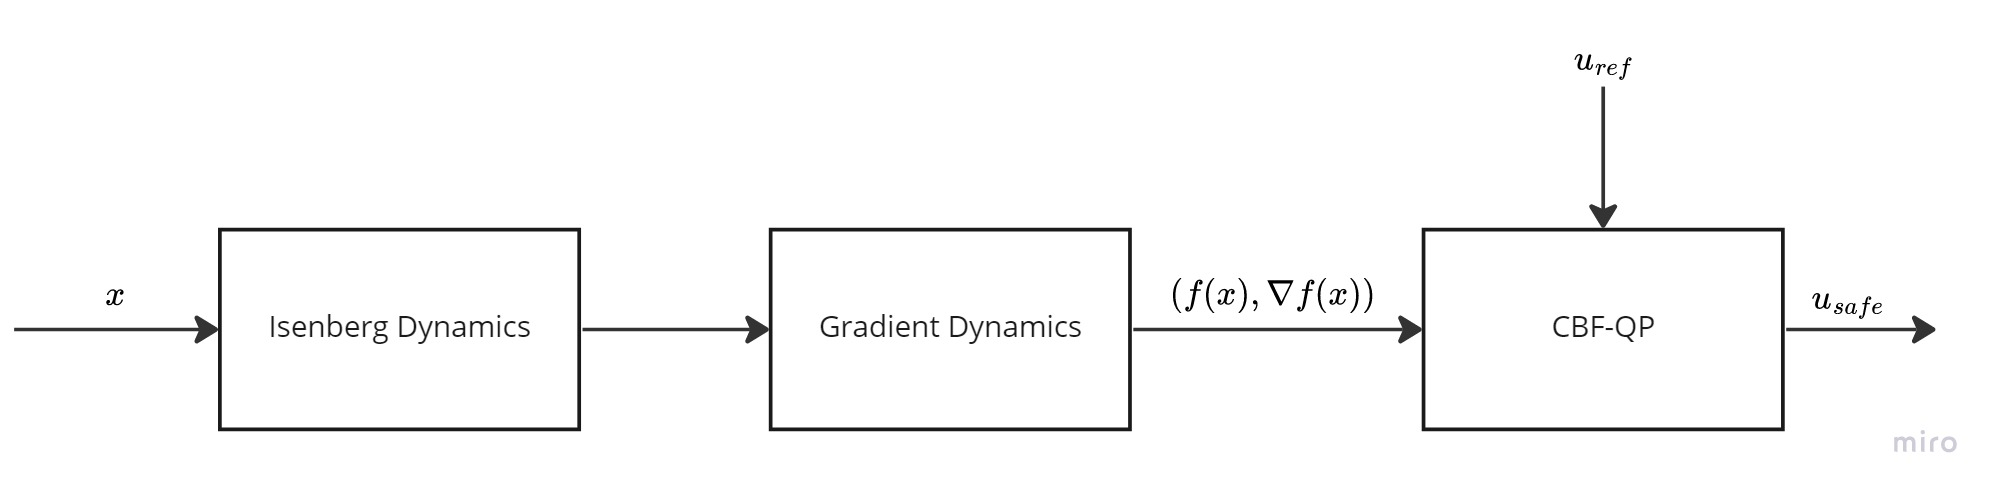
\includegraphics[width=\textwidth]{Figures/Implementation/CBFControl.jpg}
    \caption{CBF Controller with\algname{}}
    \label{fig:cbf_controller_complete}
\end{figure}

\noindent The top-level calls for an entire system are given in Algorithms \ref{alg:dyn} and \ref{alg:sys_dyn}.
\begin{algorithm}[H]
	\caption{Link Dynamics}\label{alg:dyn}
	\begin{algorithmic}
	\State $\H \gets \ZERO_{n \times n}$
	\State $\d \gets \ZERO_{n \times 1}$
	\State $\F \gets \ZERO_{n \times 1}$
	\State $\partialX{}\H \gets \ZERO_{2n \times n \times n}$
	\State $\partialX{}\d \gets \ZERO_{2n \times n}$
	\State $\partialX{}\F \gets \ZERO_{2n \times n}$
	
	\State \textbf{do} \textbf{Kinematics}
	\State \textbf{do} \textbf{Dynamics}
	\State \textbf{do} \textbf{Differential\_Kinematics}
	\State \textbf{do} \textbf{Differential\_Dynamics}
	\For {$\mathbf{c} \in \mathbf{c}_\B$}
	\State $(\H, \d,\F, \partialX{}\H, \partialX{}\d,\partialX{}\F)  $ += Link\_Dynamics($\mathbf{c}, \x, \dotx$) 
	\EndFor
	\State \Return $(\H, \d,\F, \partialX{}\H, \partialX{}\d,\partialX{}\F)$ 
	\end{algorithmic}
\end{algorithm}

\begin{algorithm}[H]
	\caption{System Dynamics}\label{alg:sys_dyn}
	\begin{algorithmic}
	\State $(\H, \d,\F, \partialX{}\H, \partialX{}\d,\partialX{}\F) \gets $ Link\_Dynamics(root, $\x, \dotx$) 
	\State $\ddotx \gets \H^{-1}\left (\F - \d \right )$
	\State $\partialX{} \ddotx \gets \H^{-1}\left (\partialX{\H} \ddotx + \partialX{\F} - \partialX{\d} \right )$
	\State $\f \gets \begin{bmatrix} \dotx & \ddotx \end{bmatrix}$
	\State $\g \gets \begin{bmatrix} \ZERO_{n \times n} & \H^{-1}\P \end{bmatrix}$
	\State $\partialX{}\f \gets \begin{bmatrix}
    \ZERO_{n \times n}  ~~~~~~ \EYE_{n \times n}  \\
    \partialX{} \ddotx 
    \end{bmatrix}$
    \State \Return $(\f, \g, \partialX{}\f)$ 
	\end{algorithmic}
\end{algorithm}
